%; whizzy paragraph -pdf xpdf -latex ./whizzypdfptex.sh
%; whizzy-paragraph "^\\\\begin{frame}\\|\\\\emtext"
% latex beamer presentation.
% platex, latex-beamer でコンパイルすることを想定。 

%     Tokyo Debian Meeting resources
%     Copyright (C) 2012 Junichi Uekawa
%     Copyright (C) 2012 Nobuhiro Iwamatsu

%     This program is free software; you can redistribute it and/or modify
%     it under the terms of the GNU General Public License as published by
%     the Free Software Foundation; either version 2 of the License, or
%     (at your option) any later version.

%     This program is distributed in the hope that it will be useful,
%     but WITHOUT ANY WARRANTY; without even the implied warreanty of
%     MERCHANTABILITY or FITNESS FOR A PARTICULAR PURPOSE.  See the
%     GNU General Public License for more details.

%     You should have received a copy of the GNU General Public License
%     along with this program; if not, write to the Free Software
%     Foundation, Inc., 51 Franklin St, Fifth Floor, Boston, MA  02110-1301 USA

\documentclass[cjk,dvipdfmx,12pt]{beamer}
\usetheme{Tokyo}
\usepackage{monthlypresentation}

%  preview (shell-command (concat "evince " (replace-regexp-in-string "tex$" "pdf"(buffer-file-name)) "&")) 
%  presentation (shell-command (concat "xpdf -fullscreen " (replace-regexp-in-string "tex$" "pdf"(buffer-file-name)) "&"))
%  presentation (shell-command (concat "evince " (replace-regexp-in-string "tex$" "pdf"(buffer-file-name)) "&"))

%http://www.naney.org/diki/dk/hyperref.html
%日本語EUC系環境の時
\AtBeginDvi{\special{pdf:tounicode EUC-UCS2}}
%シフトJIS系環境の時
%\AtBeginDvi{\special{pdf:tounicode 90ms-RKSJ-UCS2}}

\title{福岡Debian勉強会}
\subtitle{第0回 2012年2月度}
\author{岩松 信洋\\iwamatu@debian.org\\@iwamatsu}
\date{2012年2月18日}
\logo{
\includegraphics[width=8cm]{image200607/openlogo-light.eps}}

\begin{document}

\frame{\titlepage{}}

\begin{frame}{設営準備にご協力ください。}
会場設営などよろしくおねがいします。
\end{frame}

\section{Agenda}
\begin{frame}{Agenda}
\begin{minipage}[t]{0.45\hsize}
  \begin{itemize}
  \item 注意事項
	\begin{itemize}
	 \item 飲食禁止
	 \item 宗教禁止
	 \item 営利活動禁止
	\end{itemize}
   \item 最近あったDebian関連のイベント報告
	\begin{itemize}
        \item 第84回 東京エリアDebian勉強会
	\end{itemize}
 \end{itemize}
\end{minipage} 
\begin{minipage}[t]{0.45\hsize}
 \begin{itemize}
   \item Debian Trivia Quiz
   \item Debianサーバ量産工場 - 無限ポチポチ on Debian
   \item Dynamic Kernel Module Support (DKMS) Framework
   \item はじめてのGPGキーサイン&CAcert
   \item LT
   \item debhelper $\geqq 7$ での最近のパッケージング
  \end{itemize}
\end{minipage}
\end{frame}

\section{イベント報告}
\emtext{イベント報告}

\begin{frame}{第84回東京エリアDebian勉強会}
\begin{minipage}[t]{0.45\hsize}
  \begin{itemize}
  \item 注意事項
	\begin{itemize}
	 \item 飲食禁止
	 \item 宗教禁止
	 \item 営利活動禁止
	\end{itemize}
   \item 最近あったDebian関連のイベント報告
	\begin{itemize}
        \item 第83回 東京エリアDebian勉強会
	\end{itemize}
 \end{itemize}
\end{minipage} 
\begin{minipage}[t]{0.45\hsize}
 \begin{itemize}
   \item Debian Trivia Quiz
   \item Debian勉強会予約システム
   \item Debian VPS
   \item Debian で Twitterを使う
   \item 月刊Debhelper 第3回
   \item 事前課題紹介
   \item 2012年計画
  \end{itemize}
\end{minipage}
\end{frame}

\section{DWN quiz}
\emtext{DWN quiz}
\begin{frame}{Debian 常識クイズ}

Debian の常識、もちろん知ってますよね?
知らないなんて恥ずかしくて、知らないとは言えないあんなことやこんなこと、
みんなで確認してみましょう。

今回の出題範囲は\url{debian-devel-announce@lists.debian.org},
\url{debian-devel@lists.debian.org} に投稿された
内容とDebian Project Newsなどからです。

\end{frame}

\subsection{問題}
%; whizzy-master ../debianmeetingresume201201.tex
% 以上の設定をしているため、このファイルで M-x whizzytex すると、whizzytexが利用できます。
%

\santaku
{Lenny のセキュリティサポートが終わったのはいつ?}
{2012/02/06}
{2012/02/07}
{2012/02/08}
{A}
{}

\santaku
{2012/01/28 に更新された Squeeze のヴァージョンは?}
{6.0.4}
{6.1.0}
{20120128}
{A}
{}

\santaku
{Debian Game チームが 2/25から2/26まで行うイベントは何か?}
{どれだけの Windows のゲームが Wine 上で動作するか検証するパーティ}
{Debian で提供されているゲームパッケージのスクリーンショットを撮りまくるパーティ}
{Debian で提供されているゲームを48時間連続プレイするパーティ}
{B}
{}

\santaku
{Wheezy で採用される Linux カーネルヴァージョンは?}
{2.6.39}
{3.2}
{4.0}
{B}
{}

\santaku
{pts.debian.org で表示されるようになった情報は?}
{パッケージメンテナが誕生日の日は「おめでとう」と出る。}
{パッケージを乗っ取ろうとしている人の情報}
{パッケージ Transition 情報}
{C}
{}

\santaku
{アクセプトされたDEPは?}
{DEP 3}
{3 DEP }
{DEP DEP DEP}
{A}
{DEP3 は Patch tagging guideline. Debian Enhancement Proposals}




\emtext{Debianサーバ量産工場 - 無限ポチポチ on Debian}

\emtext{Dynamic Kernel Module Support Framework}
\section{Dynamic Kernel Module Support Framework}

\begin{frame}{自己紹介}

\begin{itemize}
\item 岩松 信洋 (いわまつ のぶひろ)
\item Twitter @iwamatsu
\item Debian Project Official Developer
\item Bluez(bluetooth framework), OpenCV, Mozc (Google input method), linpng(画像ファイルの)、Renesas SH4 Porter
\item U-Boot SH メンテナ
\item 普段は Linux kernel、ブートローダ開発、開発ツールのメンテナンスをしている社内ニート。
\item 実は Ruby コミッター
\end{itemize}

\end{frame}

% 本の紹介を入れる。


\begin{frame}{アジェンダ}

\begin{enumerate}
\item Dynamic Kernel Module Support Framework (DKMS)とは
\item DKMS の仕組み
\item DKMS 対応 Debian パッケージの作り方
\item DKMS Debian 対応状況
\item まとめ
\end{enumerate}
\end{frame}

\begin{frame}
\large\bfseries
\begin{center}
Dynamic Kernel Module Support Framework (DKMS)とは
\end{center}
\end{frame}

\begin{frame}{Dynamic Kernel Module Support Frameworkとは}

外部から導入した
Linux カーネルで提供されていないドライバモジュールを導入したマシンに、
インストールされているカーネル毎にドライバモジュールを管理する仕組み。

\end{frame}

\begin{frame}

\begin{itemize}
\item 使っているディストリビューションのカーネルにはまだマージされていない
ドライバを使う。
\item マージはされているが不具合があり、修正するためのパッチはまだ
マージされていない。オリジナルとは別に管理したい。
\item etc....
\end{itemize}

\end{frame}


\begin{frame}{Dynamic Kernel Module Support Frameworkとは}

\begin{itemize}
\item 通常カーネルで提供されていないドライバモジュールを使っている
場合、カーネルが更新されたとき、手動で再ビルドする必要がある。
\item DKMS はカーネルの更新を検知し、そのカーネル向けにドライバ
モジュールをビルドおよびインストールを行う。
\item 各ドライバモジュールの状態(登録、ビルド、インストール、
アンインストールなど)を管理する。
\item 特定のカーネル向けにパッチを適用できる機構などもある。
\end{itemize}

\end{frame}

\begin{frame}{Dynamic Kernel Module Support Frameworkとは}

\begin{itemize}
\item Debian や Ubuntu、Arch、Gentoo などで利用。\\
Fedora は Kmods2 という独自の実装を持っているようだ。
\item DELL が開発およびメンテナス。\\
\url{http://linux.dell.com/dkms/}
\item 今回は DKMS の仕組みと DKMS に対応したDebian パッケージの作成方法、Debian の DKMS 対応状況について説明。
\end{itemize}

\end{frame}

\begin{frame}{サンプルソースコード}

\begin{itemize}
\item 話をわかりやすくするために簡単なサンプルを使って説明。
\item ドライバをロードすると カーネルデバッグメッセージ
に「Hello, world! from hello\_init」と出力。
\item ドライバをアンロードすると「Good bye! from hello\_exit」と出力。
\item という簡単なデバイスドライバ。
\end{itemize}

\end{frame}

\begin{frame}[containsverbatim]{ドライバソースコード}
\begin{commandline}
#include <linux/init.h>
#include <linux/module.h>

static int __init hello_init(void)
{
  pr_info("Hello, world! from %s\n", __func__);
  return 0;
}

static void __exit hello_exit(void)
{
  pr_info("Good bye! from %s\n", __func__);
}

module_init(hello_init);
module_exit(hello_exit);
MODULE_LICENSE("GPL v2");
\end{commandline}

\end{frame}

\begin{frame}[containsverbatim]{ディレクトリ構成とMakfile}

ディレクトリ構成:
\begin{commandline}
hello-0.0.1
├--─Makefile
├── README
├── dkms.conf
└--src
    ├── Makefile
    └── hello.c
\end{commandline}

Makefile:
\begin{commandline}
obj-m:= src/
\end{commandline}

src/Makefile:
\begin{commandline}
obj-m:= hello.o 
\end{commandline}

\end{frame}

\begin{frame}[containsverbatim]{ドライバのコンパイルと結果}

\begin{commandline}
$ make -C /lib/modules/`uname -r`/build M=`pwd` modules
$ sudo insmod hello.ko
$ dmesg | tail -1
[5963787.044134] Hello, world! from hello_init
$ sudo rmmod hello.ko
$ dmesg | tail -1
[5963798.420368] Good bye! from hello_exit
\end{commandline}
%$
\end{frame}

\begin{frame}[containsverbatim]{dkms.conf}
\begin{commandline}
PACKAGE_NAME="hello"
PACKAGE_VERSION="0.0.1"
BUILT_MODULE_NAME="$PACKAGE_NAME"
BUILT_MODULE_LOCATION="src"
DEST_MODULE_LOCATION="/updates"
AUTOINSTALL="yes"
\end{commandline}
%$
\end{frame}

\begin{frame}
\large\bfseries
\begin{center}
DMKS の仕組み
\end{center}
\end{frame}

\begin{frame}{DKMS 全体の流れ}

\begin{center}
  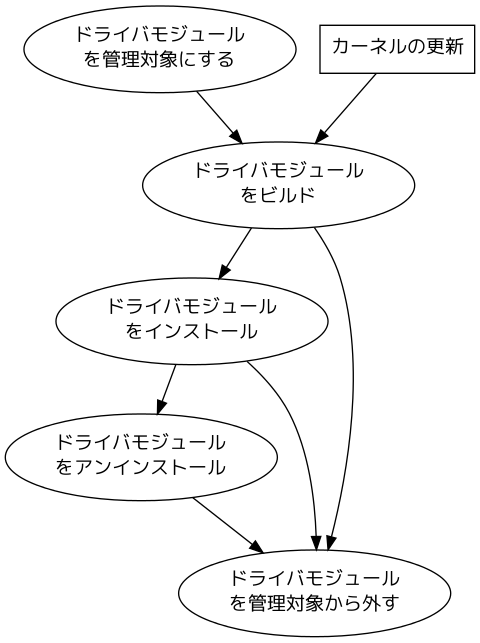
\includegraphics[width=0.5\hsize]{image201202/dkms0.png}
\end{center}

%dkms\_autoinstaller はシステム起動時に呼ばれるスクリプト。
\end{frame}

\begin{frame}[containsverbatim]{モジュールソースコードの配置位置}

DKMS 対応モジュールのソースコードは
「/usr/src/ドライバモジュール名-バージョン/」 以下に配置する必要がある。\\
先のドライバの場合、「/usr/src/hello-0.0.1/」 以下に配置する。

\begin{commandline}
$ tree /usr/src/hello-0.0.1/
/usr/src/hello-0.0.1/
├── Makefile
├── dkms.conf
└── src
    ├── Makefile
    └── hello.c

1 directory, 4 files
\end{commandline}
%$
\end{frame}

\begin{frame}{DKMS 設定ファイル}

\begin{itemize}
\item DKMS は、各ドライバパッケージ毎に設定ファイルを持つ必要がある。
\item この設定ファイルでは、どのようなドライバが提供、ビルド、インストールされるのか記述されている。
\end{itemize}

\end{frame}

\begin{frame}{DKMS 設定ファイル}

\begin{center}
  %\begin{small}

  \begin{tabular}{|l|p{17zw}|}
 \hline
 設定項目 & 内容 \\
 \hline \hline
PACKAGE\_NAME & パッケージ名 \\\hline
PACKAGE\_VERSION & パッケージバージョン \\\hline
CLEAN & キャッシュなどの一時ファイルを削除するためのコマンドを指定する。指定しない場合には "make clean" が実行される\\\hline
MAKE & モジュールをビルドするコマンドを指定する。\\
 \hline
 \end{tabular}
 %\end{small}
\end{center}

\end{frame}

\begin{frame}{DKMS 設定ファイル}

\begin{center}
  %\begin{small}

  \begin{tabular}{|l|p{13zw}|}
 \hline
 設定項目 & 内容 \\
 \hline \hline
BUILT\_MODULE\_NAME & ドライバモジュールの名前を指定する(拡張子は必要なし)。\\\hline
BUILT\_MODULE\_LOCATION &  ビルドされたモジュールが作成されるディレクトリまでの相対パス\\\hline
DEST\_MODULE\_LOCATION & モジュールをインストールするディレクトリを指定する。\\
 \hline
 \end{tabular}
 %\end{small}
\end{center}

\end{frame}


\begin{frame}{DKMS 設定ファイル}

\begin{center}
  %\begin{small}

  \begin{tabular}{|l|p{17zw}|}
 \hline
 設定項目 & 内容 \\
 \hline \hline
AUTOINSTALL & モジュールを自動的にインストールするか、"yes" か "no" を指定する。\\\hline
REMAKE\_INITRD & ドライバインストール時にINITRD イメージを再構成するか、"yes" か "no" を指定する。 \\\hline
PATCH & 適用したいパッチを指定する。\\\hline
PATCH\_MATCH & パッチを適用するバージョンの指定する。Linux カーネルが 2.6.38 と 2.6.39 の場合にパッチを適用したい場合には "2.6.(38$|$39)" と指定する。\\
 \hline
 \end{tabular}
 %\end{small}
\end{center}

\end{frame}


\begin{frame}[containsverbatim]{配列を使った指定}

\begin{itemize}
\item BUILT\_MODULE\_LOCATION や BUILT\_MODULE\_NAME などは
配列を使ってドライバモジュール毎に設定できる。
\item BUILT\_MODULE\_NAME 配列の番号は各要素の番号に紐づいているので、
処理されるときは各々の番号が参照される。
\end{itemize}
\end{frame}

\begin{frame}[containsverbatim]{配列を使った指定}

一つのドライバパッケージから foo と bar の2つのデバイスドライバ
が提供される場合:

\begin{commandline}
(省略)
BUILT\_MODULE\_NAME[0] = "foo"
BUILT\_MODULE\_LOCATION[0]  = "foo_build"
DEST\_MODULE\_LOCATION[0] = "/update"
BUILT\_MODULE\_NAME[1] = "bar"
BUILT\_MODULE\_LOCATION[1]  = "bar_build"
DEST\_MODULE\_LOCATION[1] = "/update"
(省略)
\end{commandline}

\begin{itemize}
\item ドライバ foo のビルドは 「foo\_build」 ディレクトリで行われ、
update ディレクトリ以下にインストールされる
\item ドライバ bar のビルドは
「bar\_build」 ディレクトリで行われ、update ディレクトリ以下にインストール
される。
\end{itemize}

\end{frame}

\begin{frame}{DKMS で提供されるコマンド}

DKMS は dkms コマンドで操作する。

\begin{center}
  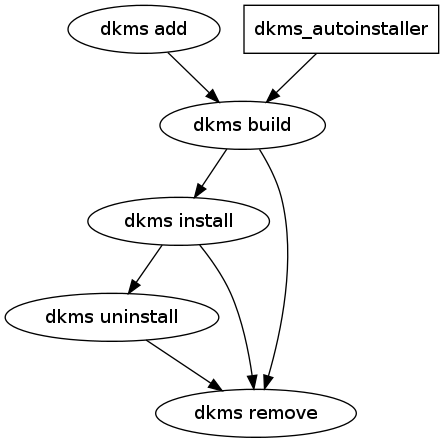
\includegraphics[width=0.6\hsize]{image201202/dkms.png}
\end{center}

\end{frame}

\begin{frame}[containsverbatim]{dkms status}

DKMS で提供されている モジュールのステータスを表示する。
\begin{commandline}
$ dkms status
v4l2loopback, 0.5.0, 3.1.0-1-amd64, x86_64: installed
v4l2loopback, 0.5.0, 3.2.0-1-amd64, x86_64: installed
virtualbox, 4.1.8, 3.1.0-1-amd64, x86_64: installed
virtualbox, 4.1.8, 3.2.0-1-amd64, x86_64: installed
\end{commandline}
%$

\end{frame}


\begin{frame}{dkms add}

\begin{center}
  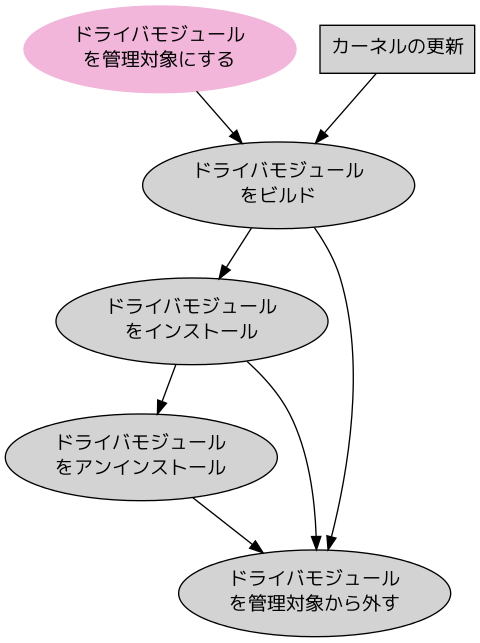
\includegraphics[width=0.5\hsize]{image201202/dkms0-add.png}
\end{center}

\end{frame}


\begin{frame}[containsverbatim]{dkms add}

\begin{itemize}
\item モジュールのソースコードを管理対象に追加する。
\item 実行時に -m オプションで追加するドライバパッケージ名を、
-v オプションでバージョンを指定する。
\end{itemize}

\begin{commandline}
$ sudo dkms add -m hello -v 0.0.1

Creating symlink /var/lib/dkms/hello/0.0.1/source ->
                 /usr/src/hello-0.0.1

DKMS: add completed.
$ dkms status
hello, 0.0.1: added
\end{commandline}
%$

実行すると/var/lib/dkms 以下に シンボリックリンクを張り、DKMS の管理
対象にする。

\end{frame}


\begin{frame}{dkms build}

\begin{center}
  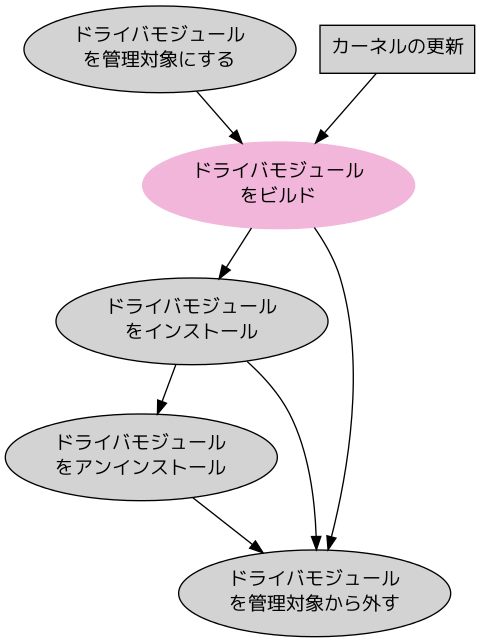
\includegraphics[width=0.5\hsize]{image201202/dkms0-build.png}
\end{center}

\end{frame}


\begin{frame}[containsverbatim]{dkms build}

\begin{itemize}
\item 管理対象になっているモジュールをビルドする。
\item 実行時に -m オプションで追加するドライバパッケージ名を、
-v オプションでバージョンを指定する。\\
\item 「/var/lib/dkms/ドライバ名/ドライババージョン/BUILT\_MODULE\_LOCATION」 ディレクトリ以下でビルドされる。\\
\item  作成されたモジュールとビルドログは
「/var/lib/dkms/ドライバ名/ドライババージョン/カーネルバージョン/アーキテクチャ」ディレクトリ
以下に置かれる。
\end{itemize}

\end{frame}



\begin{frame}[containsverbatim]{dkms build}

\begin{commandline}
$ sudo dkms build -m hello -v 0.0.1

Kernel preparation unnecessary for this kernel.  Skipping...

Building module:
cleaning build area....
make KERNELRELEASE=3.2.0-1-amd64 -C \
    /lib/modules/3.2.0-1-amd64/build \
    M=/var/lib/dkms/hello/0.0.1/build....
cleaning build area....
\end{commandline}
% $

\end{frame}


\begin{frame}{dkms install}

\begin{center}
  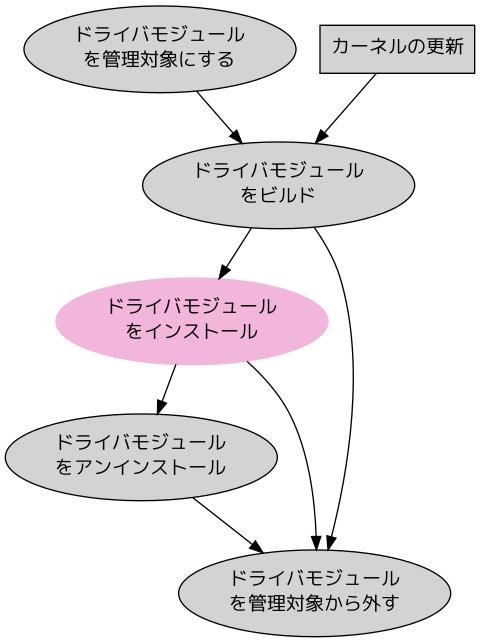
\includegraphics[width=0.5\hsize]{image201202/dkms0-install.png}
\end{center}

\end{frame}


\begin{frame}[containsverbatim]{dkms install}

\begin{itemize}
\item 「dkms build」 コマンドによってビルドされたモジュールを dkms.conf の 
DEST\_MODULE\_LOCATION で指定されている場所にインストールする。
\item Linux カーネル 3.2.0-1-amd64 を使用し、
「DEST\_MODULE\_LOCATION="/updates"」と指定されている場合、
\url{/lib/modules/3.2.0-1-amd64/updates/dkms/}
以下にインストールされる。
\end{itemize}

\end{frame}

\begin{frame}[containsverbatim]{dkms install}
\begin{commandline}
$ sudo dkms install -m hello -v 0.0.1

hello:
Running module version sanity check.
 - Original module
   - No original module exists within this kernel
 - Installation
   - Installing to /lib/modules/3.2.0-1-amd64/updates/dkms/

depmod..........

DKMS: install completed.
$ dkms status
hello, 0.0.1: installed
$ sudo modprobe -l | grep hello.ko
updates/dkms/hello.ko
\end{commandline}
%$

\end{frame}


\begin{frame}{dkms uninstall}

\begin{center}
  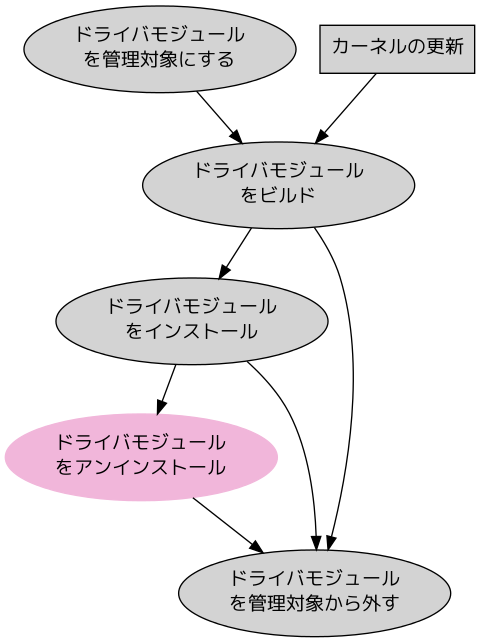
\includegraphics[width=0.5\hsize]{image201202/dkms0-uninstall.png}
\end{center}

\end{frame}


\begin{frame}[containsverbatim]{dkms uninstall}

\begin{itemize}
\item モジュールをアンインストールする。
\item 実行時に -m オプションで追加するドライバパッケージ名を、
-v オプションでバージョンを指定する。
\item 全てのカーネルから削除する場合には --all オプションを指定する。
\item 特定のカーネルバージョン向けにビルドされたモジュールを削除する場合、
-k オプションでカーネルバージョンを指定する。
\end{itemize}

\end{frame}

\begin{frame}[containsverbatim]{dkms uninstall}

\begin{commandline}
$ sudo dkms uninstall -m hello -v 0.0.1 -k 3.2.0-1-amd64

-------- Uninstall Beginning --------
Module:  hello
Version: 0.0.1
Kernel:  3.2.0-1-amd64 (x86_64)
-------------------------------------
(中略)

depmod....

DKMS: uninstall completed.
\end{commandline}
%$

NOTE: この資料を作成している時点では、「dkms uninstall」は動作しない。
一部のチェックが未実装なため、uninstall の処理まで行われないため。\\
\url{http://bugs.debian.org/cgi-bin/bugreport.cgi?bug=659672}

\end{frame}

\begin{frame}[containsverbatim]{dkms remove}

\begin{itemize}
\item DKMS の管理対象から外す。
\item uninstall と同様のオプションが必要。
\item ドライバモジュールがアンインストールされていない場合、
アンインストールを実行してから、管理対象から外される。
\end{itemize}

\end{frame}


\begin{frame}{dkms remove}

\begin{center}
  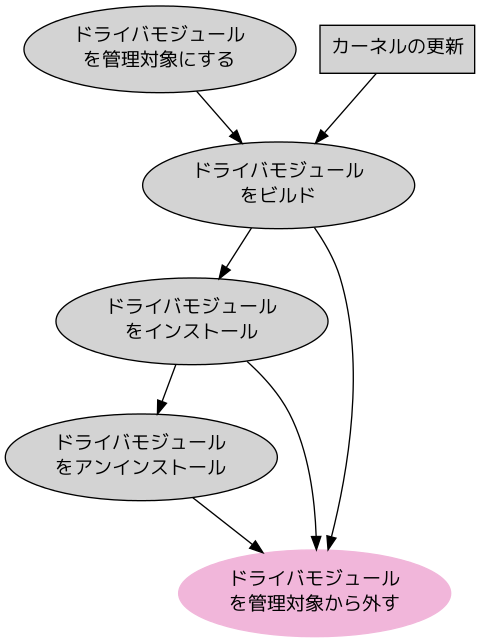
\includegraphics[width=0.5\hsize]{image201202/dkms0-remove.png}
\end{center}

\end{frame}

\begin{frame}[containsverbatim]{dkms remove}

\begin{commandline}
$ dkms status
hello, 0.0.1, 3.2.0-1-amd64, x86_64: installed
virtualbox, 4.1.6, 3.2.0-1-amd64, x86_64: installed
$ sudo dkms remove  -m hello -v 0.0.1 --all

-------- Uninstall Beginning --------
Module:  hello
Version: 0.0.1
Kernel:  3.2.0-1-amd64 (x86_64)
-------------------------------------
(中略)

depmod....

DKMS: uninstall completed.

------------------------------
Deleting module version: 0.0.1
completely from the DKMS tree.
------------------------------
Done.
$ dkms status
\end{commandline}
%$

\end{frame}

\begin{frame}[containsverbatim]{その他}

その他、rpm パッケージを作成する mkrpm オプションや Debianパッケージ
を作成する mkdeb オプションなどが用意されている。

\end{frame}

\begin{frame}
\large\bfseries
\begin{center}
DKMS 対応Debian パッケージの作り方
\end{center}
\end{frame}

\begin{frame}{DKMS 対応Debian パッケージの作り方}

\begin{itemize}
\item DKMS 対応モジュールのソースを規定のディレクトリに
展開しておくと DKMS は処理を行う。
\item Debian の場合もパッケージ化するときは
インストールした時に規定のディレクトリに展開するようにする。
\item パッケージ名などに関してはルールが決まっている。
DKMS 対応パッケージは -dkms というサフィックスがついている。\\

\begin{itemize}
\item パッケージ名が DKMS 用だとわかりやすい。
\item DKMS 用の debhelper 用コマンド、dh\_dkms コマンドが 
-dkms サフィックスのついたパッケージに対して処理を行うため。
\end{itemize}
\end{itemize}

\end{frame}


\begin{frame}{dh\_dkms}

debian/パッケージ名.dkms または debian/dkms を dkms.conf に変換して、
適切な dkms 用ディレクトリにコピーし、postinst と prerm に DKMS 用の
処理を追加する。

\end{frame}


\begin{frame}{dh\_dkms}

\begin{center}
  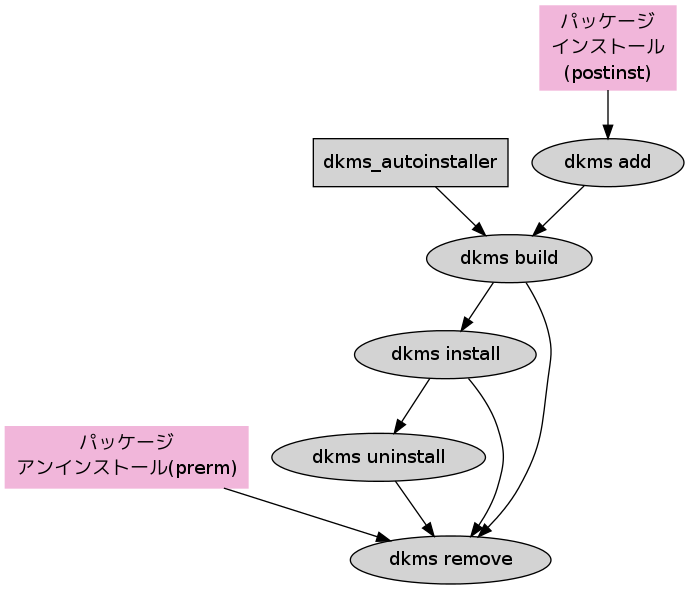
\includegraphics[width=0.8\hsize]{image201202/dkms-debian.png}
\end{center}

\end{frame}


\begin{frame}[containsverbatim]{debian/hello-dkms.dkms}

\begin{commandline}
PACKAGE_NAME="hello"
PACKAGE_VERSION="#MODULE_VERSION#"
BUILT_MODULE_NAME[0]="$PACKAGE_NAME"
BUILT_MODULE_LOCATION="src"
DEST_MODULE_LOCATION[0]="/updates"
AUTOINSTALL="yes"
\end{commandline}
%$

\begin{center}
$\downarrow$
\end{center}

\begin{commandline}
PACKAGE_NAME="hello"
PACKAGE_VERSION="0.0.1"
BUILT_MODULE_NAME[0]="$PACKAGE_NAME"
BUILT_MODULE_LOCATION="src"
DEST_MODULE_LOCATION[0]="/updates"
AUTOINSTALL="yes"
\end{commandline}
%$

\end{frame}


\begin{frame}{dh\_dkms}

dh\_dkms コマンドは dkms パッケージで提供されている。
debhelper 7 以降で利用する場合には、アドオンとして読み込ませる必要
がある。 
\end{frame}

\begin{frame}[containsverbatim]{DKMS 用 debian/rules}

\begin{commandline}
#!/usr/bin/make -f

VERSION := $(shell dpkg-parsechangelog | \
    sed -nr '/^Version:/s/Version: (.*:)?(.*)-(.*)/\2/p')

%:
    dh $@ --with dkms

override_dh_install:
    dh_install src/* usr/src/hello-$(VERSION)/src/
    dh_install Makefile usr/src/hello-$(VERSION)/
override_dh_dkms:
    dh_dkms -V $(VERSION)

override_dh_auto_configure override_dh_auto_build override_dh_auto_test \
override_dh_auto_install override_dh_auto_clean:
\end{commandline}
%$

debian/rules ファイル内で override\_dh\_auto\_configure や 
override\_dh\_auto\_build を呼び出している理由は Makefile がある場合、
make が実行されてしまうのでこれを抑制するため。

\end{frame}

\begin{frame}[containsverbatim]{Debian でのドライバモジュールビルドのタイミング}

Debian では DKMS ドライバパッケージがインストール後と、
カーネルヘッダ または カーネルイメージパッケージがインストール
(更新)後、 DKMS が起動しドライバモジュールのコンパイルが行われる。
これらは以下のファイルで処理される。

\begin{commandline}
/etc/kernel/postinst.d/dkms
/etc/kernel/header_postinst.d/dkms
\end{commandline}

ちなみにこれらは同じ内容。

\end{frame}

\begin{frame}[containsverbatim]{Debian でのドライバモジュールビルドのタイミング}

\begin{center}
  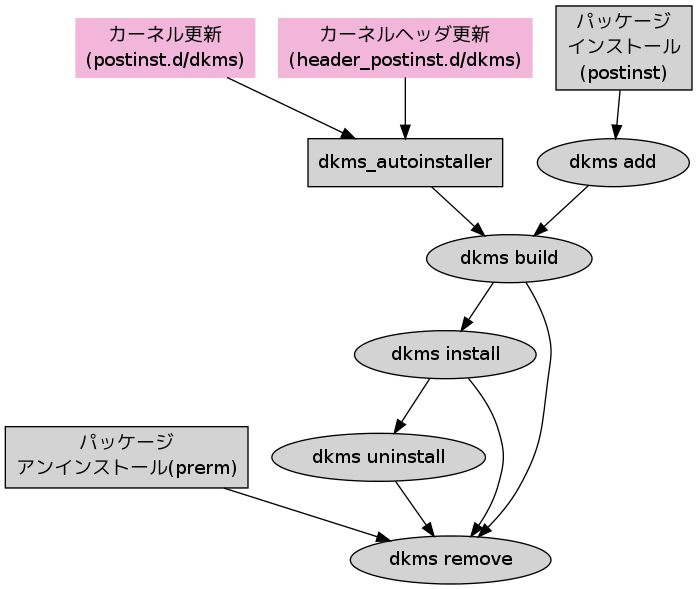
\includegraphics[width=0.8\hsize]{image201202/dkms-debian-kernel.png}
\end{center}

\end{frame}


\begin{frame}
\large\bfseries
\begin{center}
Debian DKMS 対応状況
\end{center}
\end{frame}


\begin{frame}[containsverbatim]{Debian DKMS 対応状況}

\begin{itemize}
\item メンテナンスチームがある(Debian DKMS Team)\\
\url{http://pkg-dkms.alioth.debian.org/}
\item 48個の DKMS ドライバパッケージが提供されている。
\item 主要なドライバの殆どは DKMS と module-assistant(m-a)の両方
に対応している。
\item 開発があまり活発ではないドライバは m-a のみをサポートした状態が多い。
\item 新しくパッケージ化されたドライバはほとんどが両方に対応している。
DKMS のほうがメリットが多いため、m-a から DKMS に切り替えているユーザが多いようだ。
\end{itemize}

\end{frame}

\begin{frame}[containsverbatim]{module-assistant との違い}

Debian には他のドライバパッケージ管理機構に 
module-assistant(m-a)がある。
DKMS と m-a の違いには以下のようになっている。
\begin{itemize}
\item m-a は自動ビルド機構がない。\\
カーネルが更新されるとドライバモジュールが更新されないため、手動で m-a を実行しモジュール用パッケージを作成する必要がある。
\item DMKS を使うと起動時に自動ビルドされるため、
起動に時間がかかる時がある。
\item DKMS はドライバ用のバイナリパッケージを作らない。\\
m-a は カーネル毎バイナリパッケージを作り、インストールする。
\item m-a は起動しているカーネルのみのドライバをビルドするが、DKMS は
インストールされているカーネルを対象にビルドできる。

\end{itemize}

\end{frame}


\begin{frame}
\large\bfseries
\begin{center}
まとめ
\end{center}
\end{frame}


\begin{frame}[containsverbatim]{まとめ}

\begin{itemize}

\item  DKMS の基本的な仕組みと、Debian での DKMS 対応パッケージ作成方法
について説明した。
\item DKMS Linux カーネルでサポートされていないドライバモジュールやパッチが必要な
ドライバモジュールを管理し、自動的にビルドできるシステム。
\item Debian は今までは m-a が主流だったが、DKMS もサポートしているドライバ
パッケージも増え始め、徐々に DKMS に移行しつつある。
\item Debian ではDKMS パッケージ用のチームがあり、Debian パッケージ用ツールが用意されている。DKMS 対応パッケージ作成環境は整備されている。
\item m-a と比較してメリットが大きいが、大きなドライバ(alsaなど)は起動が
遅くなることがある。
\end{itemize}

今後ドライバパッケージを作成する場合には、DKMS をサポートしてみては
いかがでしょうか。

\end{frame}


\emtext{PGP/GPG、CACert サインパーティ}

\section{PGP/GPG、CACert サインパーティ}

\begin{frame}{アジェンダ}
\begin{itemize}
\item PGP/GPG とは?
\item 使い所
\item キーサインの流れ
\item キーサイン
\end{itemize}
\end{frame}

\begin{frame}{PGP/GPG とは?}
  \begin{itemize}[<+->]
    \item PGP/GPG は公開鍵暗号方式 
    \item $\rightarrow$ 公開鍵を本当に実在する人間が管理しているものなのか、保証してもらう必要がある
    \item しかし 証明書のように PGP/GPG には認証局が無い
    \begin{itemize}
      \item 自分が相手を保証して、相手が自分を保証する\\
      \item これをPGP/GPGユーザで相互に行う $\rightarrow$ ネットワークが構築される $\rightarrow$ Web of Trust
    \end{itemize}
    \item 実際に会って、相手の公開鍵と公的ID(パスポート、運転免許証)を確認、そして公開鍵に署名=キーサイン
    \item 誰とも鍵交換してない GPG 署名なんて何の意味を持たない\\
          だって誰にも信頼されてないじゃない.....。
    \item 多くの人と鍵を交換している人と署名すると効率的。
  \end{itemize}
\end{frame}

\begin{frame}{使い所: 開発者}

\begin{itemize}
  \item 存在証明
  \begin{itemize}
    \item 公開サーバのアカウント認証など
  \end{itemize}
  \item ソフトウェアのリリース署名、リポジトリの署名チェック
  \begin{itemize}
    \item Debian、Ubuntu の開発では必須
    \item パッケージへの署名、投票の署名...
  \end{itemize}
  \item Linux カーネル開発(Linus に pull してもらう場合)でも必須に。
\end{itemize}
\end{frame}

\begin{frame}{使い所: ユーザ}
\begin{itemize}
  \item メールの署名/暗号化
  \item データファイルの署名
  \item ソフトウェアの改竄チェック
  \begin{itemize}
    \item リポジトリの署名チェック(apt, yum etc..)
  \end{itemize}
\end{itemize}
\end{frame}


\begin{frame}
  \begin{center}

これらを行うには Web of Trust に参加している必要がある \\ \pause
\Huge\bfseries 
というわけで、キーサインしましょう。
  \end{center}
\end{frame}

\begin{frame}{キーサインの流れ}
\begin{enumerate}
  \item キーサーバに自分の公開鍵をアップロード
  \item 相手の確認(名前、公開鍵の指紋, ID、メールアドレス)
  \item 相手の公開鍵に署名(メールアドレス毎に!)
  \item 署名した相手に公開鍵を送信(メールアドレス毎に!)
  \item 相手に署名された自分の鍵を取り込む
  \item キーサーバに自分の公開鍵をアップロード
\end{enumerate}
\end{frame}

\begin{frame}{あるキーサインパーティ前のWoT}
\begin{center}
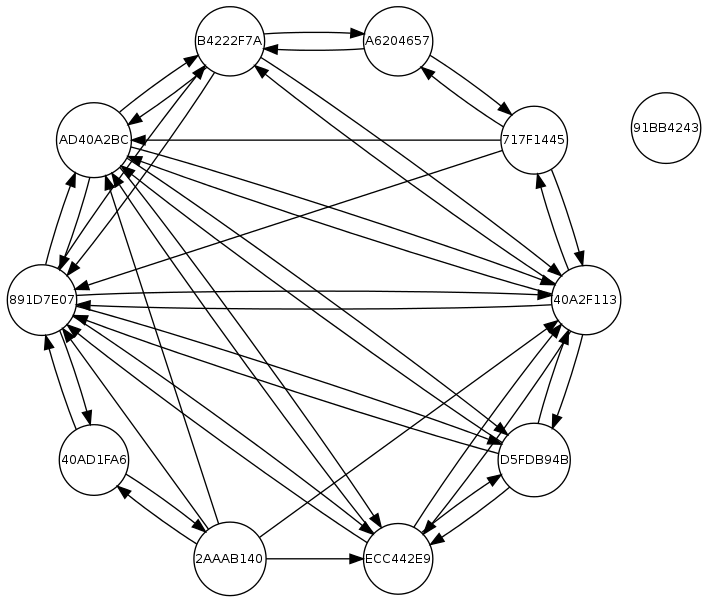
\includegraphics[width=0.8\hsize]{image201111/kof2011-ksp.png}
\end{center}
\end{frame}


\begin{frame}{あるキーサインパーティ後のWoT}
\begin{center}
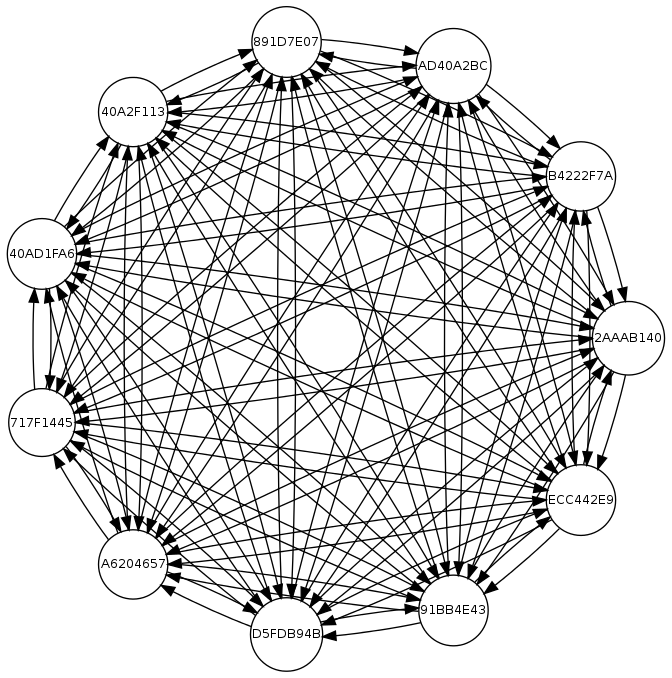
\includegraphics[width=0.7\hsize]{image201111/kof2011-ksp0.png}
\end{center}
\end{frame}

\begin{frame}{GPG サインパーティ後}

\begin{itemize}
\item 相手にサインして送るまでが PGP/GPG サイン。
\item caff を使うと楽ちんです。
\end{itemize}

\end{frame}


\emtext{Debian JP Project \& 祝Debianサーバ in 福岡}

\section{今後のイベント}
\emtext{今後のイベント}
\begin{frame}{今後のイベント}
 
\begin{itemize}
 \item 3月 OSC Tokyo Spring\\
  展示とセミナー。内容は未定。
 \item 第1回 福岡 Debian 勉強会 ?
\end{itemize}
\end{frame}

\section{今日の宴会場所}
\begin{frame}{今日の宴会場所}

\begin{center}
 {\Large 未定}
\end{center}
\end{frame}

\end{document}

;;; Local Variables: ***
;;; outline-regexp: "\\([ 	]*\\\\\\(documentstyle\\|documentclass\\|emtext\\|section\\|begin{frame}\\)\\*?[ 	]*[[{]\\|[]+\\)" ***
;;; End: ***


